\chapter{nftables}

\texttt{nftables}\footnote{\url{https://netfilter.org/projects/nftables/index.html}} è la soluzione di nuova generazione per il firewalling in
Linux, il cui intento è quello di sostituire iptables.
In questo capitolo si analizza come funziona nftables, come e perché è migliore
del suo predecessore, e soprattutto, come si è passati da iptables a nftables
sia lato server sia lato client.

\section{Prerequisiti}
Prima di spiegare nftables si procede ad introdurre in maniera rigorosa iptables,
questo consentirà di comprendere meglio come mai nftables sia superiore.

\paragraph{netfiler}
\textit{netfilter} è il componente del kernel Linux che
``\textit{enables packet filtering, network address [and port] translation
(NA[P]T) and other packet mangling}'', il quale viene utilizzato mediante il
popolare programma iptables (ed \textit{ip6tables}, \textit{arptables},
\textit{ebtables})\footnote{\url{https://netfilter.org/index.html}}. Si tratta di una strumento molto
potente, che consente a qualsiasi dispositvo supportato dal kernel Linux
di diventare un firewall (o di compiere praticamente qualsiasi altra operazione
sui pacchetti in transito).\\
Sia netfilter sia iptables si scrivono senza maiuscole.


netfilter è composto da una serie di \textit{hook} a cui è possibile registrare
delle \textit{callback} che sono chiamate ogni volta che un pacchetto passa per
un certo hook. \cite{digitalocean-iptables} \\
Un pacchetto che entra in contatto con lo stack di rete di Linux transita per
diverse parti di esso in diversi momenti; un hook non è un altro che un \textit{punto} dello stack
in cui il pacchetto passa.
L'intero stack di rete offre numerosi hook, e non tutti sono disponibili in netfilter.
In particolare, quelli disponibili sono:
\begin{itemize}
  \item \texttt{NF\_IP\_PREROUTING}, raggiunto da tutti i pacchetti appena entrano nello
  stack di rete, la decisione di routing deve ancora essere presa.
  \item \texttt{NF\_IP\_LOCAL}, per i pacchetti dopo che sono stati \textit{routed}
  dal sistema e destinati al sistema locale.
  \item \texttt{NF\_IP\_FORWARD}: dopo che si è presa la decisione di routing,
  per pacchetti \textit{in transito} ad un altro sistema.
  \item \texttt{NF\_IP\_LOCAL\_OUT}: pacchetti creati localmente e destinati ad
  altri sistemi (quindi viene dopo la decisione di routing).
  \item \texttt{NF\_IP\_POSTROUTING}, raggiunto da tutto i pacchetti dopo che
  sono stati \textit{routed} e stanno per uscire dal sistema.
  \item \texttt{NF\_IP\_INGRESS} è un hook disponibile nelle versioni più recenti di
  Linux, avviene prima di \texttt{NF\_IP\_PREROUTING} per pacchetti in ingresso.
  E' utile per il cosìdetto ``\textit{early packet dropping}''\cite{netfilter-hooks}.
\end{itemize}

\begin{figure}
  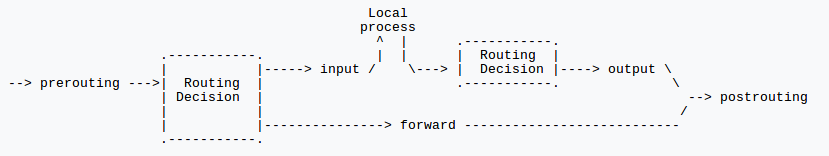
\includegraphics[scale=0.5]{img/NetfilterHooks}
  \caption[Hook di netfiler]{Gli hook di netfilter \textit{classici}. Tutti i
  pacchetti in arrivo passano per \texttt{PREROUTING}, viceversa quelli in
  uscita devono passare per forza per \texttt{POSTROUTING}.
  \url{https://wiki.nftables.org/wiki-nftables/index.php/Netfilter_hooks}}
  \label{fig:netfiler-hooks}
\end{figure}


\begin{figure}
  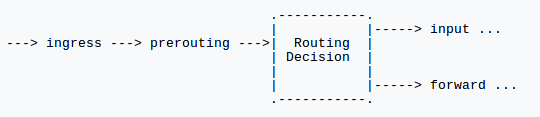
\includegraphics[scale=0.5]{img/NetfilterIngress}
  \caption[Hook \texttt{INGRESS}]{Hook \texttt{INGRESS} di Netfilter. E' l'hook
  che viene prima di tutti gli altri.
  \url{https://wiki.nftables.org/wiki-nftables/index.php/Netfilter_hooks}}
  \label{fig:ingress-hooks}
\end{figure}

\paragraph{iptables}
iptables è uno dei programmi userspace usati per registrare degli hook in netfilter e
specificare quale azioni devono essere eseguite.  Ciò che tipicamente si scrive
mediante iptables sono delle \textit{regole}, esse sono organizzate in
\textit{tabelle}, le quali a loro volta sono costituite da \textit{chain}. Esistono delle
tabelle predefinite:
\begin{itemize}
  \item \texttt{filter}: utilizzata per definire regole di firewalling
  \item \texttt{mangle}: usata per generiche modifiche ai pacchetti
  \item \texttt{nat}: utilizzata la traduzione NAT/PAT
  \item \texttt{raw}: utilizzata principalmente per operare sui pacchetti senza
  il tracking della connessione (più veloce)
  \item \texttt{security}: per distribuzioni che sfruttano \texttt{SELinux}
\end{itemize}
E' possibile definire delle tabelle ulteriori.
Le chain predefinite sono:
\begin{itemize}
  \item \texttt{FORWARD} per pacchetti che passano attraverso
  il sistema
  \item \texttt{INPUT} per i pacchetti ricevuti e destinati al sistema locale
  \item \texttt{OUTPUT}: pacchetti generati dal sistema in uscita da esso
  \item \texttt{PREROUTING} per operare su pacchetti appena arrivano nello
  stack di rete
  \item \texttt{POSTROUTING} per lavorare su pacchetti quando stanno per uscire
  dal sistema.
\end{itemize}
Non tutte le tabelle hanno a disposizione tutte le chain, ad esempio nella tabella
di \texttt{nat} vi sono \texttt{PREROUTING} e \texttt{POSTROUTING}, mentre
in \texttt{filter} è possibile usare \texttt{INPUT}, \texttt{FORWARD}, \texttt{OUTPUT}.\\
Come si può dedurre dal nome delle chain, esse corrispondono agli hook di
netfilter:

\begin{table}[h]\label{tbl:iptables-chain}
  \begin{tabular}{|c|c|}
    \hline
    Hook & Chain \\
    \hline
    \hline
    \texttt{NF\_IP\_PREROUTING} & \texttt{PREROUTING}\\
    \hline
    \texttt{NF\_IP\_LOCAL} & \texttt{INPUT}\\
    \hline
    \texttt{NF\_IP\_FORWARD} & \texttt{FORWARD}\\
    \hline
    \texttt{NF\_IP\_LOCAL\_OUT} & \texttt{OUTPUT}\\
    \hline
    \texttt{NF\_IP\_POSTROUTING} & \texttt{POSTROUTING}\\
    \hline
  \end{tabular}
  \caption[La corrispondenza tra gli hook di netfilter e le chain di iptables.]
  {La corrispondenza tra gli hook di netfilter e le chain di iptables; si può notare
  come non sia possibile usare l'hook \texttt{NF\_IP\_INGRESS} perché non disponibile in
  iptables.}
\end{table}


\paragraph{Regole}
Le regole iptables sono composte da due parti: una parte detta di \textit{match}
nella quale si specificano i criteri per cui un pacchetto matcha o meno una regola,
ed una seconda di \textit{target} (indicato con l'opzione \texttt{-j}) che specifica quale
\textit{azione} compiere per quel pacchetto se vi è matching. Alcune tra i
target disponibili sono:
\begin{itemize}
  \item \texttt{ACCEPT} per accettare il pacchetto
  \item \texttt{DROP} per droppare il pacchetto, eliminandolo ed impedendo che
  prosegua nel suo attraversamento del kernel
  \item \texttt{REJECT} per droppare il pacchetto inviando un pacchetto
  \texttt{ICMP} al mittente
  \item \texttt{DNAT} per la traduzione NAT/PAT modificando l'indirizzo
  IP/porta destinazione
  \item \texttt{SNAT} per la traduzione NAT/PAT dell'indirizzo/porta sorgente.
\end{itemize}


Un'importante funzionalità offerta da netfilter è il tracking della connessione
in una tabella di stato (nota come ``\textit{Connection Tracking}''), che è la base
per il NAT e stateful firewalling.\\
Infine, sono disponibili numerose estensioni sia per matching sia per target;
ad esempio, esiste una versione di iptables
(\textit{iptables L7}) che aggiunge comprensione anche dei protocolli
applicativi\footnote{\url{http://l7-filter.clearos.com/start}}.
iptables viene usato con il protocollo IP versione 4 (e protocolli di livello
superiore che si appoggiano ad IPv4), se si vuole lavorare con protocolli
di livello 3 diversi, o protocolli di livello inferiore vi sono:
\begin{itemize}
  \item \texttt{arptables}: manipolazione di pacchetti ARP
  \item \texttt{ebtables} per lavorare con frame Ethernet
  \item \texttt{ip6tables} per pacchetti che usano IPv6 come protocollo di rete.
\end{itemize}

\section{Criticità}
Ogni volta che si invoca un comando in \textit{userspace} per modificare il set
di regole, tale programma ottiene dal kernel il \textit{blob}
di \textit{tutte} le regole, vi applica le modifiche, invia la versione
modificata al kernel.
Questo porta a numerosi problemi, tra cui il fatto che più il numero di regole
aumenta, più la modifica delle regole è lenta.
Si vorrebbe un'aggiunta delle regole in batch ed \textit{atomica}, che
sia al contempo più veloce ed affidabile.

Ci sono vari altri problemi con iptables che negli anni sono emersi, e la
maggior parte di essi non sono attualmente risolvibili se non con un grosso
cambio a livello progettuale, cambio che non è possibile perché richiederebbe
dei \textit{breaking changes}, e vista la vasta diffusione di iptables questo
non è possibile.
Alcuni dei problemi sono:
\begin{description}
  \item[Duplicazione del codice]Per ogni protocollo gestito da iptables (o sue
  controparti), occorre che vi sia comprensione di esso sia a livello
  utente (perché il programma in \textit{userspace} deve creare il \textit{blob} per
  il kernel), sia a livello di \textit{kernelspace}, per operare correttamente sul pacchetto
  secondo quanto specificato dall'utente.\\
  Ciò significa che \textit{per ogni nuovo protocollo}, esso deve essere
  supportato sia in \textit{userspace} sia in \textit{kernelspace}.
  \item[Target multipli]Si supponga che si voglia loggare un pacchetto
  \textit{e} dropparlo, in una sola regola non è possibile, è necessario, ad
  esempio, creare una nuova tabella.
  \item[Matching avanzato]Se non si usano estensioni per ogni match si può specificare
  un solo valore per un certo campo. Ad esempio si può definire un match che controlli
  sia la porta TCP mittente sia quella del destinatario, ma comunque si
  deve specificare \textit{un solo} valore con cui fare match, \textit{solo} una porta mittente
  e \textit{solo} una destinatario.
  Quindi, se si vuole scrivere una regola che abiliti il traffico in entrata verso
  le porte 80 e 443 bisogna scrivere due regole, poiché vi sono due valori per uno stesso campo.
  % \item[Matching avanzato]iptables supprta matching controllando l'header
  % del protocollo di trasporto e l'header IP, tuttavia non è possibile scrivere
  % in una \textit{regola} il fatto che il traffico TCP sulla porta 8 \textit{e}
  % 443 sono consentite: occore scrivere almeno due regole. Questo diventa
  % particolarmente tedioso quando il numero di regole aumenta molto (esistono
  % estensioni come \texttt{multiport} per il matching di porte multiple, ma ne
  % supporta solo fino a 15).
  \item[Multipli programmi]Un'altra criticità è il fatto che vi sono 4 programmi
  \textit{userspace} diversi, particolarmente problematica è la gestione separata di IPv4
  e IPv6.
  \item[Scalabilità]Come si comporta iptables/netfilter quando vi sono
  davvero molte regole (centinaia o più) regole da gestire ed il troughput
  è elevatissimo? La risposta è purtroppo semplice, iptables non scala, a causa
  del suo design che prevede l'attraversamento delle varie regole.
\end{description}

Questi problemi hanno portato gli sviluppatori di netfilter ad introdurre
una nuova soluzione, molto più avanzata \cite{nftables-pro}.

\section{nftables}

%TODO BPF REF
La soluzione a questi problemi c'è e si chiama \texttt{nftables}.
Esso utilizza un approccio completamente diverso rispetto ai predecessori: una
\textit{in-kernel virtual machine} per il packet matching, concettualmente
simile a \texttt{BPF -- Berkeley Packet Filter}.
Vi è un unico programma in userspace chiamato
\texttt{nft}, il quale traduce in bytecode i comandi inseriti dall'utente e li
\textit{inietta} nel kernel (mediante \texttt{Netlink}\footnote{\texttt{Netlink}
	è un meccanismo IPC -- Inter-Process Comunication del kernel Linux che consente
	di comandare e ottenre informazioni riguardo lo stack di rete, è una interfaccia
che offre API basate su socket.}). Ecco un elenco
delle principali novità:
\begin{itemize}
	\item Il kernel non ha più conoscenza specifica
	      dei protocolli di rete: fare match con una porta TCP o un flag dell'header Ethernet
	      si traduce in semplici istruzioni come: \textit{carica x byte del pacchetto nel
	      registro z a partire dall'offset y}. Questo significa che è molto facile estendere
	      nftables con nuovi protocolli, e che il codice del kernel è molto più semplice.
	\item Non ci sono tabelle e chain di default.
	\item Ogni regola consente di pià target in una sola volta.
	\item Il programma \texttt{nft} diventa l'unico programma per la gestione delle regole,
	      rimpiazzando iptables, ip6tables, arptables, ebtables.
	\item L'aggiunta, l'aggiornamento, la cancellazione ed ogni altra operazione
	      sulle regole viene ora fatta in maniera atomica. Ciò significa che ogni volta che
	      si fa un'operazione, anche su più regole, essa va a buon fine (cioè i suoi effetti
	      sono applicati) solo se ogni singola operazione va a buon fine.
	\item Possibilità di gestire contemporanemente IPv4 ed IPv6 in una singola tabella/chain.
	\item Supporto a strutture dati avanzate basate su \texttt{set} che consentono un matching/targeting
	      molto veloce.
	\item La sintassi delle regole cambia e diventa più simile ad una frase.
\end{itemize}

La maggior parte dell'\textit{intelligenza} è spostata su \texttt{nft}, il quale compila
le regole ricevute in input e le passa al kernel, esso è anche responsabile di
decompilare il bytecode presente nel kernel per presentarlo all'utente in un
formato human-readable.

Vi sono due tipi di sintassi supportate: il primo è una sintassi assimilabile a quella
di iptables dove si scrive una regola per volta. Il secondo tipo è invece
una sintassi \textit{strutturata} più simile a sintassi usati in specifici
file di configurazione. Saranno mostrati esempi di entrambe.


\paragraph{Tabelle e chain}
Si è detto che non esistono tabelle di default, quindi è spetta all'utente
il compito di crearle. In nftables, le tabelle sono di una certa \textit{famiglia}:
\begin{itemize}
	\item \texttt{ip} è la famiglia per operare su pacchetti dal livello 3 in su e
	      che usano IPv4 come protocollo di rete; è la famiglia di default se non è specificata.
	\item \texttt{ip6} è la famiglia per operare con pacchetti di protocolli che utilizzano
	      il protocollo IPv6.
	\item \texttt{arp} viene utilizzata per processare pacchetti ARP.
	\item \texttt{inet} è la famiglia che consente di lavorare con pacchetti sia IPv4
	      sia IPv6.
	\item \texttt{bridge} è usata per lavorare con frame Ethernet.
	\item \texttt{netdev} consente di \textit{attaccarsi} direttamente ad una interfaccia
	      di rete.
\end{itemize}
Le tabelle sono solo dei contenitori vuoti, il cui nome non ha alcuna semantica (rispetto
ad iptables). Comunque, la scelta della famiglia influenza quali hook possono
essere utilizzati (es: l'hook \texttt{ingress} è disponibile solo per \texttt{netdev}).

Le tabelle a loro volta racchiudono delle chain, ed anche in questo caso non vi
sono delle chain predefinite ma occorre crearle. Quando si crea una chain occorre
specificare
almeno tre cose:
\begin{itemize}
	\item tipo; le scelte possibili sono:
	      \begin{itemize}
	      	\item \texttt{filter} da utilizzare quando si vuole fare del filtraggio
	      	\item \texttt{nat} per utilizzare le funzionalità NAT
	      	\item \texttt{route} per fare generico \textit{packet mangling} che non sia NAT
	      \end{itemize}
	\item hook, in questo caso le scelte possibili sono gli hook già visti, cambia solo
	      il fatto che vengono scritti in minuscolo.
	\item priorità: espressa con un numero, si tratta di una priorità \textit{inversa},
	      più è bassa più il suo valore è alto; indica l'ordine con cui alcune operazioni
	      sono svolte. Un \textit{buon} valore è 0.
\end{itemize}

Quando si crea una nuova chain è possibile specificare la policy di default, cioè
l'azione da compiere se non si matcha nessun'altra regola; il valore di default è
\texttt{accept} (accettazione il pacchetto), altri valori possibili sono: \texttt{drop},
\texttt{queue}, \texttt{continue}, \texttt{return}.


\subsection{Set e altre strutture dati}
nftables introduce tre strutture dati pensate indirizzando i problemi
presenti in iptables (e sue controparti):
\begin{itemize}
	\item matching limitato, per cui è problematico specificare più di una porta
	      o più di un singolo indirizzo IP in una regola; il che porta a:
	\item elevato numero di regole a causa della suddetta limitazione.
\end{itemize}
E' possibile dichiarare queste strutture dati in due modi:
\begin{itemize}
	\item \textit{anonymous}: vengono create ed istanziate all'interno di una regola
	      e sono immutabili, non è possibile modificarle dopo la loro creazione.
	\item \textit{Named}: sono vere e proprie variabili che vivono nello \textit{scope}
	      di una tabella in cui sono definite. Una volta create è possibile modificarle
	      in seguito. Per riferirsi ad una variabile, occorre preporre \texttt{@} al nome
	      della variabile.
\end{itemize}
L'idea principale che sta dietro le strutture dati di nftables  è quella di poter
ridurre drasticamente il numero di regole necessarie. Migliorie che si sono
dimostrate efficaci; per una dettagliata comparazione delle performance tra
iptables e nftables si veda \cite{nftables-iptables-thesis}.

\subsubsection{Set}
La struttura dati avanzata di nftables si chiama \textit{set}, ed è implementata
utilizzando alberi rosso-neri, tabelle di hash, bitmap.
Un set è, come dice il nome, un insieme di elementi di un certo \textit{tipo},
esso può essere un tipo \textit{base} predefinito come \texttt{ipv4\_addr} o
\texttt{inet\_service} (porta protocollo di trasporto), oppure un tipo complesso
\textit{composto} da altri tipi, ad esempio un nuovo tipo \texttt{ipv4\_port}.
Quando si crea una nuova struttura dati è possibile specificare vari parametri,
tra cui una \texttt{policy}: per cosa deve essere ottimizzata la struttura?
I valori possibili sono \texttt{performance} o \texttt{memory}
Un esempio è il seguente.

I set sono utilizzati per:
\begin{itemize}
	\item fare match su più elementi in un unico regola, ad esempio, se si vogliono
	      bloccare connessioni da 10 indirizzi IP diversi, è possibile definire un set
	      che contenga questi 10 IP, anziché scrivere 10 regole diverse. Si consideri che
	      i set sono molto performanti.
	\item Essere la struttura dati base su cui si creano ulteriori strutture dati.
\end{itemize}


\subsubsection{Map}
Le map sono costruite sui set, infatti possono essere visti come dei set in cui
ciascun elemento è composto a sua volta da due elementi: il primo di essi
è la \textit{chiave}, il secondo è il \textit{valore} associato alla chiave. Essi
si comportano effettivamente come una mappa poiché definiscono un \textit{mappaggio}
tra la chiave ed il valore, e sono utilizzati in contesti in cui si \textit{trasforma}
un input in un certo output secondo il mappaggio definito in questa struttura dati.
Si può forse intuire l'utilizzo delle map nel mappaggio delle reti\ldots


In particolare, le map sono molto utili con target di tipo \texttt{dnat} ed \texttt{snat}.
Si supponga che si voglia modificare l'indirizzo IP destinazione da \texttt{192.168.1.0/24}
nel corrispondente indirizzo in \texttt{192.168.100.0/24} (mantenendo lo stesso
offset) in \texttt{prerouting}, ed il viceversa in \texttt{postrouting}. Si
è già visto che farlo in iptables richiede 508 regole, 254 per ogni indirizzo in
\texttt{prerouting} e 254 per ogni indirizzo in \texttt{postrouting}. Con nftables
lo si può fare in due regole e due mappe!
L'esempio qui riportato mostra come farlo, ed è esattamente ciò che è stato fatto
nella mia soluzione finale di mappaggio delle reti (si veda la sezione successiva
per maggiori dettagli).


\subsubsection{Dictionary}
La struttura dati \textit{dictionary}, a vole nota anche come \textit{vmap -- verdict map}
, è concettualmente
molto simile alle map, tuttavia gli elementi di questo insieme sono nelle forma:
\texttt{key: verdict}, dove \texttt{Verdict} indica l'azione da applicare nel
momento in cui si la chiave viene
matchata.

\paragraph{Esempi}
Di seguito si riportano degli esempi che mostrano il funzionamento di nftables.
Si noti in particolare come, nelle ultime quattro regole l'utilizzo dei set
consente di specificare match multipli in un'unica regola. Questo non significa
solo una comodità per chi scrive le regole, infatti i set sono molto performanti
e sono le strutture dati base su cui nftables costruisce altre strutture
più avanzate, che verranno descritte in seguito.

Supponendo che ciò che si vede listato qui sotto sia il contenuto di un file,
si può notare lo shebang all'inizio, in modo che sia eseguito da nft nella
modalità nativa di shell che offre: tutte queste regole sono inserite atomicamente
in una transazione. Invocando questi comandi in una shell normale invece si
perderebbe l'atomicità perché ciascun comando è una invocazione separata al programma nft
(si noti che qui tutte le regole non sono appunto prefisse da ``\textit{nft}'').
% BIG WARNING: state {related, established} and state related,established seems to be the same
\begin{minted}{squidconf}
	#!/usr/sbin/nft -f
	
	# creazione della tabella, sia IPv4 sia IPv6
	# chiamata 'filter'
	add table inet filter
	
	# aggiunta chain 'input'
	add chain inet filter input { type filter hook input priority 0; \
	policy drop;}
	
	# chain 'output'
	add chain inet filter output { type filter hook output priotrity 0; \
	policy drop;}
	
	# consentire il traffico in entrata sulla porta 22 in modo statefull
	add rule inet filter input tcp dport 22 ct state\
	new, related, established accept
	
	# consentire le risposte
	add rule inet filter output tcp sport 22 ct state\
	related, established accept
	
	# consentire tutto il traffico in uscita sulle
	# porte 80 e 443 usando un set
	add rule inet output tcp dport { 80, 443 } ct state \
	new, related, established accept
	
	# consentire le risposte
	add rule input tcp sport { 80, 443 } ct state \
	related, established accept
	
	# creazione di un set chiamato 'allowed'
	
	add set filter allowed { type: ipv4_addr }
	add element filter allowed {
		192.168.1.20,
		192.168.2.20,
		192.168.100.1,
		192.168.200.254,
		10.7.0.20
	}
	
	# consentire tutte le connessioni dagli indirizzi IP
	# elencati sulla porta 8080
	# nota: per accedere ad una named set si utilizza '@'
	add rule input ip saddr @allowed tcp dport 8080 \
	ct state {new, related, established } accept
	# consentire le risposte
	add rule output ip daddr @allowed tcp sport 8080 \
	ct state {related, established }accept
\end{minted}
E' possibile ottenere lo stesso risultato usando una sintassi \textit{strutturata}:
\begin{minted}{squidconf}
	#!/usr/sbin/nft -f
	table inet filter {
		set allowed {
			type ipv4_addr
			elements = {
				192.168.1.20,
				192.168.2.20,
				192.168.100.1,
				192.168.200.254,
				10.7.0.20
			}
		}
		
		chain input {
			type inet hook input priority 0; policy drop;
			tcp dport 22 ct state new, related, established accept
			tcp sport {80, 443} ct state {related, established accept
				ip saddr @allowed tcp dport 8080 ct state new, related,
				established accept
			}
			
			chain output {
				type inet hook output priority 0; policy drop;
				tcp sport 22 ct state related, established accept
				tcp dport {80, 443}  ct state new, related, established accept
				ip addr @allowed tcp sport 8080 ct state elated,
				established accept
			}
		}
	\end{minted}
	Per ottenere la lista delle regole attive, è disponibile il comando
	\texttt{nft list ruleset}, che produce un output nello stesso formato \textit{strutturato}
	apppena mostrato.
	
	L'esempio seguente si concentra invece sull'utilizzo dei dizionari.
	Si supponga di dover gestire una serie di regole relative alla porta 22:
	\begin{itemize}
		\item consentito dalle reti \texttt{192.168.100.0/24}, \texttt{192.168.101.0/24},
		      \texttt{192.168.200.0/24}
		\item proveniente dalla rete \texttt{192.168.1.0/24} occorre \texttt{REJECT}
		\item tutto il resto non è consentito.
	\end{itemize}
	\begin{minted}[breaklines]{bash}
		iptables -t filter -A INPUT -p tcp --dport 22 -s 192.168.100.0/24 -j ACCEPT
		iptables -t filter -A INPUT -p tcp --dport 22 -s 192.168.101.0/24 -j ACCEPT
		iptables -t filter -A INPUT -p tcp --dport 22 -s 192.168.200.0/24 -j ACCEPT
		
		iptables -t filter -A INPUT -p tcp --dport 22 -s 192.168.1.0/24 -j REJECT
		iptables -t filter -A INPUT -p tcp --dport 22 -j DROP
		
		# per brevità le regole in OUPUT sono omesse
	\end{minted}
	Mentre con nftables:
	\begin{minted}{squidconf}
		#!/usr/sbin/nft -f
		
		# supponendo tabelle e chain già create
		# aggiunta di 'dict' alla tabella filter
		add map filter dict { type ipv4_addr: verdict; }
		
		add element filter dict { 192.168.100.0/24: accept, \
			192.168.101.0/24: accept, \
			192.168.200.0/24: accept, \
		192.168.1.0/24: reject }
		
		add rule filter input tcp dport 22 ip saddr vmap @dict
		add rule filter input tcp dport 22 drop
	\end{minted}

\section{Come è stato usato}
Si supponga di voler gestire un VPN client che gestisce una singola rete classe C:
con il vecchio approccio di iptables, come guà detto, sono necessarie esattamente
19 regole:
\begin{itemize}
  \item 254 per trasformare gli indirizzi IP mappati negli indirizzi IP originali
  \item 254 regole per trasformare gli IP originali negli IP mappati
  \item 1 per gestire il \textit{NAT al contrario}
\end{itemize}
nftables è stato adottato prima che si conducessero veri test sul campo
in cui si potessero misurare le performance della soluzione basata su iptables,
quindi
non è stato possibile determinare quale fosse la scalabilità effettiva della vecchia
proposta, certo è che con con nftables \textit{si riduce il numero di regole
da 19 a 3}! Non solo, le nuove regole sono create utilizzando strutture
dati performanti, e sono e rimangono sempre 3, a prescindere che si il client VPN
rimappi una o $n$ reti.

In particolare si è sfruttata la struttura dati \textit{map} proprio come è stata
descritta nella sezione precedente. Si definiscono due \textit{named maps},
una per la gestione
del \texttt{PREROUTING} chiamata \texttt{remapping}, ed una per il \texttt{POSTROUTING}
chiamata \texttt{mapping}. La ragione per cui si sono scelte delle \textit{named maps}
è che consentono di essere modificate in seguito, per cui per qualsiasi eventualità
un operatore può agire direttamente su esse lasciando intatte le regole.
Di seguito un esempio, supponendo la seguente configurazione:
\begin{itemize}
  \item $OTN$: \texttt{192.168.100.0/24}
  \item $MTN$: \texttt{192.168.1.0/24}
  \item subnet VPN: \texttt{10.7.0.0/24}
\end{itemize}
Il file di script per nftables viene creato usando la sintassi \textit{strutturata},
di seguito se ne riporta, per brevità, solo un estratto.
\begin{minted}{squidconf}
#!/usr/sbin/nft -f
table ip ovpn_nat {

  map mapping {
    type ipv4_addr: ipv4_addr
    elements = {
      192.168.1.1: 192.168.100.1,
      192.168.2.1: 192.168.100.2,
      192.168.1.3: 192.168.100.3,
      192.168.1.4: 192.168.100.4,
      192.168.1.5: 192.168.100.5,
      192.168.1.6: 192.168.100.6,
      192.168.1.8: 192.168.100.8,
      192.168.1.9: 192.168.100.9,
    }
  }

  map remapping {
    type ipv4_addr: ipv4_addr
    elements = {
      192.168.100.1: 192.168.1.1,
      192.168.100.2: 192.168.1.2,
      192.168.100.3: 192.168.1.3,
      192.168.100.4: 192.168.1.4,
      192.168.100.5: 192.168.1.5,
      192.168.100.6: 192.168.1.6,
      192.168.100.7: 192.168.1.7,
      192.168.100.8: 192.168.1.8,
      192.168.100.9: 192.168.1.9      
    }
  }

  chain prerouting {
    type nat hook prerouting priority 0; policy accept;
    ip saddr 10.7.0.0/24 dnat to ip addr map @remapping
  }

  chain postrouting {
    type nat hook postrouting priority 0; policy accept;
    ip saddr 10.7.0.0/24 ip daddr 192.168.100.0/24 masquerade
    ip daddr 10.7.0.0/24 snat to ip saddr map @mapping
  }
}
\end{minted}


% TODO speak about the two nft formats
